\documentclass[12pt]{report}
\usepackage[spanish]{babel}
\usepackage[utf8]{inputenc}
\usepackage{amsmath}
\usepackage{amssymb}
\usepackage{amsthm}
\usepackage[mathscr]{euscript}
\usepackage{graphics}
\usepackage{wrapfig}
\usepackage{subfigure}
\usepackage{lipsum}
\usepackage{array}
\usepackage{multicol}
\usepackage{enumerate}
\usepackage[framemethod=TikZ]{mdframed}
\usepackage[a4paper, margin = 1.5cm]{geometry}
\usepackage{bbm}
\usepackage{float}
\usepackage{enumitem}

%En esta parte se hacen redefiniciones de algunos comandos para que resulte agradable el verlos%

\renewcommand{\theenumii}{\roman{enumii}}

\def\proof{\paragraph{Demostración:\\}}
\def\endproof{\hfill$\blacksquare$}

\def\sol{\paragraph{Solución:\\}}
\def\endsol{\hfill$\square$}

%En esta parte se definen los comandos a usar dentro del documento para enlistar%

\newtheoremstyle{largebreak}
  {}% use the default space above
  {}% use the default space below
  {\normalfont}% body font
  {}% indent (0pt)
  {\bfseries}% header font
  {}% punctuation
  {\newline}% break after header
  {}% header spec

\theoremstyle{largebreak}

\newmdtheoremenv[
    leftmargin=0em,
    rightmargin=0em,
    innertopmargin=-2pt,
    innerbottommargin=8pt,
    hidealllines = true,
    roundcorner = 5pt,
    backgroundcolor = gray!60!red!30
]{exa}{Ejemplo}[section]

\newmdtheoremenv[
    leftmargin=0em,
    rightmargin=0em,
    innertopmargin=-2pt,
    innerbottommargin=8pt,
    hidealllines = true,
    roundcorner = 5pt,
    backgroundcolor = gray!50!blue!30
]{obs}{Observación}[section]

\newmdtheoremenv[
    leftmargin=0em,
    rightmargin=0em,
    innertopmargin=-2pt,
    innerbottommargin=8pt,
    rightline = false,
    leftline = false
]{theor}{Teorema}[section]

\newmdtheoremenv[
    leftmargin=0em,
    rightmargin=0em,
    innertopmargin=-2pt,
    innerbottommargin=8pt,
    rightline = false,
    leftline = false
]{propo}{Proposición}[section]

\newmdtheoremenv[
    leftmargin=0em,
    rightmargin=0em,
    innertopmargin=-2pt,
    innerbottommargin=8pt,
    rightline = false,
    leftline = false
]{cor}{Corolario}[section]

\newmdtheoremenv[
    leftmargin=0em,
    rightmargin=0em,
    innertopmargin=-2pt,
    innerbottommargin=8pt,
    rightline = false,
    leftline = false
]{lema}{Lema}[section]

\newmdtheoremenv[
    leftmargin=0em,
    rightmargin=0em,
    innertopmargin=-2pt,
    innerbottommargin=8pt,
    roundcorner=5pt,
    backgroundcolor = gray!30,
    hidealllines = true
]{mydef}{Definición}[section]

\newmdtheoremenv[
    leftmargin=0em,
    rightmargin=0em,
    innertopmargin=-2pt,
    innerbottommargin=8pt,
    roundcorner=5pt
]{excer}{Ejercicio}[section]

%En esta parte se colocan comandos que definen la forma en la que se van a escribir ciertas funciones%

\newcommand\abs[1]{\ensuremath{\left|#1\right|}}
\newcommand\divides{\ensuremath{\bigm|}}
\newcommand\cf[3]{\ensuremath{#1:#2\rightarrow#3}}
\newcommand\natint[1]{\ensuremath{\left[\!\left[ #1\right]\!\right]}}
\newcommand{\afa}{\:
    \begin{tikzpicture}
        \draw [line width = 0.17 mm, black] (0,0) -- (-0.115,0.29);
        \draw [line width = 0.17 mm, black] (0,0) -- (0.115,0.29);
        \draw [line width = 0.17 mm, black] (-0.12,0) arc (190:-10:0.12cm);
    \end{tikzpicture}
    \:
}
\newcommand{\bbm}[1]{\mathbbm{#1}}
\newcounter{figcount}
\setcounter{figcount}{1}
%Este símvolo es para casi todo salvo una cantidad finita

%recuerda usar \clearpage para hacer un salto de página

\begin{document}
    \setlength{\parskip}{5pt} % Añade 5 puntos de espacio entre párrafos
    \setlength{\parindent}{12pt} % Pone la sangría como me gusta
    \title{Notas Taller Topología Algebraica}
    \author{Cristo Daniel Alvarado}
    \maketitle

    \tableofcontents %Con este comando se genera el índice general del libro%

    \setcounter{chapter}{1} %En esta parte lo que se hace es cambiar la enumeración del capítulo%
    
    \chapter{Grupos Libres y Productos de Grupos Libres}
    
    En los capítulos siguientes será indispensable el tratar con grupos libres, dada la naturaleza del grupo fundamental de los espacios topológicos. Para ello, primero daremos una introducción de conceptos previos para poder llegar a la definición formal de grupos libres.\\
    
    \section{Producto Débil de Grupos}
    
    \begin{obs}
        De ahora en adelante, el símbolo $\afa$ significa \textit{para casi todo salvo una cantidad finita de elementos}.
    \end{obs}

    \begin{obs}
        En esta parte, $I$ no denotará al intervalo $[0,1]$, sino a una indexación de una familia.
    \end{obs}

    \begin{mydef}
        Sea $\mathcal{G}=\left\{G_i \right\}_{ i\in I}$ una familia arbitraria no vacía de grupos. Se define el \textbf{producto directo de la familia $\mathcal{G}$} por:
        \begin{equation*}
            \prod\mathcal{G}=\left\{\cf{x}{I}{\prod_{ i\in I}G_i}\Big|x\textup{ es función} \right\}
        \end{equation*}
        y en ocasiones se denotará simplemente por $\prod_{ i\in I}G_i$. Se dota a este conjunto de la siguiente operación: si $x,y\in\prod\mathcal{G}$, entonces $\cf{x\cdot y}{I}{\prod_{ i\in I}G_i}$ es la función tal que
        \begin{equation*}
            (x\cdot y)(i)=x(i)\cdot y(i)
        \end{equation*}
        para todo $i\in I$, siendo la multiplicación respectiva en cada grupo.
    \end{mydef}

    En caso de que no lo haya hecho, queda como ejercicio al lector probar que el producto directo de una familia de grupos $\mathcal{G}$ es un grupo dotado de la operación de la definición anterior.

    \begin{mydef}
        Sea $\mathcal{G}=\left\{G_i \right\}_{ i\in I}$ una familia arbitraria no vacía de grupos. Se define el \textbf{producto débil de la familia $\mathcal{G}$} como el subgrupo de $\prod\mathcal{G}$ dado por:
        \begin{equation*}
            \prod\mathcal{G}^*=\left\{x\in\prod\mathcal{G}\Big|x(i)=e_i,\afa i\in I \right\}
        \end{equation*}
        donde $e_i$ denota la identidad de $G_i$ para cada $i\in I$.
    \end{mydef}

    \begin{propo}
        Si $\mathcal{G}$ es una familia arbitraria no vacía de grupos, entonces
        \begin{equation*}
            \prod\mathcal{G}^*<\prod\mathcal{G}
        \end{equation*}
        es decir, que $\prod\mathcal{G}^*$ es un subgrupo de $\prod\mathcal{G}$.
    \end{propo}

    \begin{proof}
        Ejercicio.
    \end{proof}

    \begin{mydef}
        Sea $\mathcal{G}=\left\{G_i \right\}_{ i\in I}$ una familia no vacía de grupos. Si $G_i$ es abeliano para cada $i\in I$, entonces llamaremos a $\prod\mathcal{G}^*$ la \textbf{suma directa de los grupos $G_i$}. En este caso, se denotará la operación del grupo de forma aditiva y se le denotará por:
        \begin{equation*}
            \prod\mathcal{G}^*=\bigoplus_{ i\in I}G_i=\bigoplus\mathcal{G}
        \end{equation*}
    \end{mydef}

    \begin{obs}
        Note que ambas definiciones coinciden si $I$ es un conjunto finito.
    \end{obs}

    \begin{mydef}
        En las condiciones de la definición anterior, para cada índice $i\in I$ definimos un \textbf{monomorfismo natural} $\cf{\varphi_i}{G_i}{\prod\mathcal{G}^*}$ definido como sigue: $\forall g\in G_i$ y para todo $j\in I$:
        \begin{equation*}
            \varphi_i(g)_j(\varphi_i(g))(j)=\left\{
                \begin{array}{lcr}
                    g & \textup{ si } & i = j\\
                    e_j & \textup{ si } & i\neq j\\
                \end{array}
            \right.
        \end{equation*}
    \end{mydef}

    En el caso en que cada $G_i$ sea un grupo abeliano, el siguiente teorema da una caracterización importante de su producto débil y de los monomorfismos $\varphi_i$.

    \begin{theor}
        \label{caractSumDir_1}
        Si $\left\{G_i \right\}_{ i\in I}$ es una familia no vacía de grupos abelianos y,
        \begin{equation*}
            G=\bigoplus_{ i\in I}G_i
        \end{equation*}
        entonces para cualquier grupo abeliano $A$ y cualquier familia de homomorfismos $\left\{\psi_i\right\}_{ i\in I}$ tales que
        \begin{equation*}
            \cf{\psi_i}{G_i}{A},\quad\forall i\in I
        \end{equation*}
        Existe un único homomorfismo $\cf{f}{G}{A}$ tal que para todo $i\in I$ el siguiente diagrama es conmutativo:

        \begin{minipage}{\textwidth}
            \begin{center}
                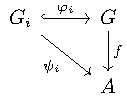
\includegraphics[scale=1.5]{images/fig_1.pdf}\\
                Figura \thefigcount. Diagrama conmutativo de $G$ y $A$.
                \stepcounter{figcount}
            \end{center}
        \end{minipage}

        esto es, $f\circ\varphi_i=\psi_i$ para todo $i\in I$.
    \end{theor}

    \begin{proof}
        Sean $A$ un grupo abeliano y $\left\{\psi_i\right\}_{ i\in I}$ una familia de homomorfismos tales que
        \begin{equation*}
            \cf{\psi_i}{G_i}{A},\quad\forall i\in I
        \end{equation*}
        sea ahora $x\in G$, como $x_i=e_i,\afa i\in I$ se tiene pues al ser $\psi_i$ homomorfismos debe suceder que $\psi_i(x_i)=e_A,\afa i\in I$ (siendo $e_A$ la identidad de $A$). Por lo cual la suma
        \begin{equation*}
            \sum_{ i\in I}\psi_i(x_i)
        \end{equation*}
        está bien definido (pues solo una cantidad finita de estos elementos es diferente de la identidad). Hacemos
        \begin{equation*}
            f(x)=\sum_{ i\in I}\psi_i(x_i),\quad\forall x\in G
        \end{equation*}
        Veamos que esta función está bien definida, ya se tiene por lo anterior que $\cf{f}{G}{A}$. Sea $x\in G$, si $x$ se expresa como
        \begin{equation*}
            x=\sum_{ j=1}^n y_j \quad\textup{y}\quad x=\sum_{ k=1}^m z_k
        \end{equation*}
        con $y_j,z_k\in G$ para todo $j\in\natint{1,n}$ y para todo $k\in\natint{1,m}$, sea
        \begin{equation*}
            I_0=\left\{i_1,...,i_r \right\}
        \end{equation*}
        el subconjunto de $I$ tal que si $i\in I_0$, entonces
        \begin{equation*}
            {y_j}_i\neq e_i\quad\textup{o}\quad{ z_k}_i\neq e_i 
        \end{equation*}
        para algún $j\in\natint{1,n}$ o algún $k\in\natint{1,m}$. Veamos que
        \begin{equation*}
            \begin{split}
                f\left(\sum_{ j=1}^n y_j \right)&=\sum_{ i\in I}\psi_i\left(\left(\sum_{ j=1}^n y_j\right)_i\right)\\
                &=\sum_{ i\in I_0}\psi_i\left(\sum_{ j=1}^n {y_j}_i\right)\\
                &=\sum_{ i\in I_0}\sum_{ j=1}^n \psi_{ i}\left( {y_j}_{i}\right)\\
            \end{split}
        \end{equation*}
        y,
        \begin{equation*}
            \begin{split}
                f\left(\sum_{ k=1}^m z_k \right)&=\sum_{ i\in I}\psi_i\left(\left(\sum_{ k=1}^m z_k\right)_i\right)\\
                &=\sum_{ i\in I_0}\psi_i\left(\sum_{ k=1}^m {z_k}_i\right)\\
                &=\sum_{ i\in I_0}\sum_{ k=1}^m \psi_{ i}\left( {z_k}_{i}\right)\\
            \end{split}
        \end{equation*}
        por ende,
        \begin{equation*}
            \begin{split}
                f\left(\sum_{ j=1}^n y_j \right)-f\left(\sum_{ k=1}^m z_k \right)&=\sum_{ i\in I_0}\sum_{ j=1}^n \psi_{ i}\left( {y_j}_{i}\right)-\sum_{ i\in I_0}\sum_{ k=1}^m \psi_{ i}\left( {z_k}_{i}\right)\\
                &=\sum_{ i\in I_0}\left(\sum_{ j=1}^n \psi_{ i}\left( {y_j}_{i}\right)-\sum_{ k=1}^m \psi_{ i}\left( {z_k}_{i}\right)\right)\\
                &=\sum_{ i\in I_0}\left(\psi_{ i}\left(\sum_{ j=1}^n {y_j}_{i}\right)-\psi_{ i}\left(\sum_{ k=1}^m{z_k}_{i}\right)\right)\\
                &=\sum_{ i\in I_0}\left(\psi_{ i}\left(\sum_{ j=1}^n {y_j}_{i}\right)-\psi_{ i}\left(\sum_{ k=1}^m{z_k}_{i}\right)\right)\\
                &=\sum_{ i\in I_0}\left(\psi_{ i}\left(\sum_{ j=1}^n {y_j}_{i}-\sum_{ k=1}^m{z_k}_{i}\right)\right)\\
            \end{split}
        \end{equation*}
        %TODO Algo falta aquí sobre la conmutatividad de los $G_i$
        pero $x_i=\sum_ { j=1}^n {y_j}_i$ y $x_i=\sum_ { k=1}^m {z_k}_i$, por lo cual
        \begin{equation*}
            \begin{split}
                f\left(\sum_{ j=1}^n y_j \right)-f\left(\sum_{ k=1}^m z_k \right)&=0\\
                \Rightarrow f\left(\sum_{ j=1}^n y_j \right)&=f\left(\sum_{ k=1}^m z_k \right)\\
            \end{split}
        \end{equation*}
        Se sigue que $f$ está bien definida. Veamos que es homomorfismo. Sean $x,y\in G$, entonces
        \begin{equation*}
            \begin{split}
                f(x+y)&=\sum_{ i\in I}\psi_i(x_i+y_i)\\
                &=\sum_{ i\in I}\psi_i(x_i)+\psi_i(y_i)\\
            \end{split}
        \end{equation*}
        como $A$ es abeliano, esta suma se puede reordenar de cualquier forma, en particular:
        \begin{equation*}
            \begin{split}
                f(x+y)&=\sum_{ i\in I}\psi_i(x_i)+\psi_i(y_i)\\
                &=\sum_{ i\in I}\psi_i(x_i)+\sum_{ i\in I}\psi_i(y_i)\\
                &=f(x)+f(y)\\
            \end{split}
        \end{equation*}
        por lo que $f$ es homomorfismo. Sea ahora $i\in I$, entonces
        \begin{equation*}
            \begin{split}
                f\circ\varphi_i(x_i)&=f(\varphi_i(x_i))\\
                &=\sum_{ j\in I}\psi_j({\varphi_i(x_i)}_j)\\
                &=\psi_i({\varphi_i(x_i)}_i)\\
                &=\psi_i(x_i),\quad\forall x_i\in G_i\\
            \end{split}
        \end{equation*}
        Luego, $f\circ\varphi_i=\psi_i$ para todo $i\in I$. Veamos la unicidad. Para ello, recordemos antes que si $x\in G$, entonces
        \begin{equation*}
            x=\sum_{ i\in I}\varphi_i(x_i)
        \end{equation*}
        (básicamente $x$ se expresa como la suma de sus componentes una por una vistas como elementos de $G$) siendo esta suma finita y por ende, está bien definida. Si $\cf{g}{G}{A}$ es otro homomorfismo tal que
        \begin{equation*}
            g\circ\varphi_i=\psi_i,\quad\forall i\in I
        \end{equation*}
        se tiene que
        \begin{equation*}
            \begin{split}
                g(x)&=g\left(\sum_{ i\in I}\varphi_i(x_i)\right)\\
                &=\sum_{ i\in I} g\circ\varphi_i(x_i)\\
                &=\sum_{ i\in I}\psi_i(x_i)\\
                &=f(x),\quad\forall x\in G\\
            \end{split}
        \end{equation*}
        por ende, $f$ es único.
    \end{proof}

    Este teorema caracteriza la suma directa de grupos abelianos, como lo muestra la siguiente proposición.

    \begin{propo}
        \label{caractSumDir_2}
        Sea $\left\{G_i \right\}_{ i\in I}$ una familia de grupos abelianos y $G=\bigoplus_{ i\in I}G_i$; sea $G'$ un subgrupo abeliano y consideremos para cada $i\in I$ las funciones $\cf{\varphi_i'}{G_i}{G'}$ tales que la conclusión del Teorema \ref{caractSumDir_1} cambiando a $G'$  y $\varphi_i'$ por $G$ y $\varphi_i$, respectivamente. Entonces, existe un único isomorfismo $\cf{h}{G}{G'}$ tal que el siguiente diagrama:
        
        \begin{minipage}{\textwidth}
            \begin{center}
                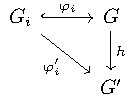
\includegraphics[scale=1.5]{images/fig_3.pdf}\\
                Figura \thefigcount. Diagrama conmutativo de $G$ y $G'$.
                \stepcounter{figcount}
            \end{center}
        \end{minipage}

        es conmutativo, para todo $i\in I$.
    \end{propo}

    \begin{proof}
        La existencia de un único homomrfismo $\cf{h}{G}{G'}$ que haga que el diagrama anterior sea conmutativo es inmediata del Teorema \ref{caractSumDir_1}. Por este mismo teorema, existe un único homomorfismo $\cf{k}{G'}{G}$ tal que el siguiente diagrama es conmutativo, para todo $i\in I$ (cambiando los papeles de $G'$ por $G$ y de $\varphi'$ por $\varphi_i$):
        
        \begin{minipage}{\textwidth}
            \begin{center}
                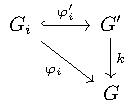
\includegraphics[scale=1.5]{images/fig_4.pdf}\\
                Figura \thefigcount. Diagrama conmutativo de $G'$ y $G$.
                \stepcounter{figcount}
            \end{center}
        \end{minipage}

        Se sigue de estos dos diagramas que:
        \begin{equation*}
            (k\circ h)\circ\varphi_i=\varphi_i\quad\textup{y}\quad(h\circ k)\circ\varphi_i'=\varphi_i'
        \end{equation*}
        para todo $i\in I$, estamos diciendo que los diagramas:
        
        \begin{minipage}{\textwidth}
            \begin{center}
                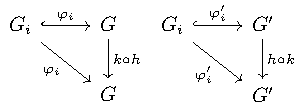
\includegraphics[scale=1.5]{images/fig_5.pdf}\\
                Figura \thefigcount. Diagramas conmutativos de $G$ y $G'$.
                \stepcounter{figcount}
            \end{center}
        \end{minipage}

        son conmutativos. Notemos que estos también son conmutativos cambiando a $k\circ h $ por $\bbm{1}_G$ y lo mismo cambiando a $h\circ k$ por $\bbm{1}_{G'}$. Como estos homomorfismos son únicos (tanto $h$ como $k$), debe suceder que:
        \begin{equation*}
            k\circ h=\bbm{1}_G\quad\textup{y}\quad h\circ k=\bbm{1}_{G'}
        \end{equation*}
        por ende, $h$ es isomorfismo.
    \end{proof}

    La importancia de este teorema, es que si consideremos un grupo abeliano $A$ como un \textit{producto} de grupos abelianos $G_i$, entonces el teorema anterior asegura que $G$ (el producto débil de los $G_i$) es el \textit{más libre} de entre todos los candidatos en el sentido de que existe un homomorfismo de $G$ en $A$ que conmuta con $\varphi_i$ y $\psi_i$, para todo $i\in I$.

    En este sentido, usamos la palabra \textit{más libre} como \textit{la menor cantidad de relaciones impuestas} (realmente podemos hablar en un sentido más particular, aterrizando la noción de objetos libres en una categoría, pero resulta complicado establecerla sin amplio conocimiento previo de Teoría de Categorías), y la filosofía general es es que si ciertas relaciones se cumplen para el grupo $G$, entonces éstas también deberan cumplirse en cualquier imagen homomorfa de $G$.

    Este mismo tipo de filosofía se matiene para otras estructuras algebraicas, como lo son los anillos, módulos, etc\dots

    Como el producto débil $G$ de subgrupos esta totalmente caracterizado por los monomomorfismos $\varphi_i$ de $G_i$ en $G$, podemos dejar de pensar que el producto débil es un subgrupo del grupo
    \begin{equation*}
        \prod_{ i\in I}G_i
    \end{equation*}
    y más aún, podemos pensar a los grupos $G_i$ como conjuntos en $G$ bajo la imagen de $\varphi_i$.

    \section{Grupos Abelianos Libres}

    Recordemos que si $G$ es un grupo, decimos que un conjunto $S\subseteq G$ \textbf{genera a $G$}, si
    \begin{equation*}
        G=\left\{s_1^{\epsilon_1}\cdot\dots\cdot s_m^{\epsilon_m}\Big|s_i\in S,\epsilon_i\in\left\{-1,1\right\}, \forall i\in\natint{1,m}; m\in\mathbb{N} \right\}
    \end{equation*}
    y en tal caso, se denota $G=\langle S\rangle$. 

    \begin{exa}
        Si $G$ es un grupo cíclico de orden $n\in\mathbb{N}$, entonces existe $x\in G$ tal que $G=\langle x\rangle$, así que
        \begin{equation*}
            G=\left\{x,x^2,...,x^n=e\right\}
        \end{equation*}
    \end{exa}

    Si un conjunto $S$ genera a un grupo, entonces ciertos productos de elementos de $S$ pueden coincidir con la identidad de $G$, por ejemplo:
    \renewcommand{\theenumi}{\alph{enumi}}
    \begin{enumerate}
        \item Si $x\in S$, entonces $xx^{-1}=e_G$.
        \item Si $G$ es un grupo cíclico de orden $n$ generado por $\left\{x\right\}$, entonces $x^n=1$.
    \end{enumerate}

    Cualquier producto de elementos de $S$ que sea igual a la identidad del grupo es llamado una \textbf{relación}.

    Distinguiremos dos tipos de relaciones: \textbf{relaciones triviales} (como las del inciso (a)) y \textbf{relaciones no triviales} (como las del inciso (b)).

    Estas nociones dan lugar a la siguiente definición:

    \begin{mydef}
        Sea $S\subseteq G$ un conjunto de generadores del grupo $G$. Decimos que $G$ es \textbf{libremente generado} por $S$, o \textbf{grupo libre en $S$}, si no hay relaciones no triviales entre los elementos de $S$.
    \end{mydef}

    \begin{exa}
        Si $G$ es un grupo cíclico infinito, entonces $G$ es un grupo libre en el conjunto $S=\left\{x \right\}$.
    \end{exa}

    Estas nociones dan lugar a la idea de que podemos caracterizar totalmente a un grupo $G$ enlistando sus elementos de un conjunto generador $S$, y las relaciones no triviales que se cumplen entre ellos.
    
    El problema de caracterizar estas ideas de esta forma, es que carecen de rigor matemático, pues ¿qué significa ser una \textit{relación no trivial}?

    Con la formación de la teoría de categorías, se fueron formalizando estas ideas y actualmente no se describe a un grupo libre de la forma en que se hace en la definición anterior. Para describirlo de una forma rigurosa, se hace uso de las siguientes dos observaciones:

    \renewcommand{\theenumi}{\arabic{enumi}}
    \begin{enumerate}
        \item Sea $S$ un conjunto de generadores de $S$, y sea $\cf{f}{G}{G'}$ un epimomorfismo, esto es que $G'$ es la imagen homomorfa de $G$. Entonces, el conjunto $f(S)$ es un conjunto de generadores de $G'$. Más aún, \textit{cualquier relación entre los elementos de $S$ se mantiene entre los elementos de $f(S)$ correspondientes}. Entonces, el grupo $G'$ satisface las mismas relaciones (o inclusive más) que el grupo $G$.
        \item Sea $S$ un conjunto de generadores de $G$, y sea $\cf{f}{G}{G'}$ un homomorfismo arbitrario. Entonces, $f$ está completamente determinado por su reestricción a $S$. Pero, no cualquier función $\cf{g}{S}{G'}$ puede ser extendida a un homomorfismo. La razón intuitiva es que dada la función $g$, puede que las relaciones que se cumplían en $S$ no se siguan cumpliendo en $g(S)$.
    \end{enumerate}

    \begin{exa}
        Considere $\mathbb{Z}$ y sea $\cf{g}{\left\{1\right\}}{\mathbb{Z}}$ dada por:
        \begin{equation*}
            g(1)=2
        \end{equation*}
        entonces, $g$  no puede ser extendida a un homomorfismo de $\mathbb{Z}$ en sí mismo.
    \end{exa}

    Con estas condiciones en mente, daremos una definición formal de lo que significa que un grupo \textit{abeliano} (se hará primero este caso, pues es el más sencillo de entender) sea libre.


    \begin{mydef}
        Sea $S$ un conjunto arbitrario. Un \textbf{grupo abeliano libre} en el conjunto $S$ es un grupo abeliano $F$ junto con una función $\cf{\varphi}{S}{F}$ tal que se cumple la siguiente condición:
        \begin{itemize}
            \item Para cualquier grupo abeliano y cualquier función $\cf{\psi}{S}{A}$, existe un único homomorfismo $\cf{f}{F}{A}$ tal que el diagrama:
            
            \begin{minipage}{\textwidth}
                \begin{center}
                    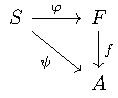
\includegraphics[scale=1.5]{images/fig_2.pdf}\\
                    Figura \thefigcount. Diagrama conmutativo de $G$ y $A$.
                    \stepcounter{figcount}
                \end{center}
            \end{minipage}
            
            es conmutativo.
        \end{itemize}
    \end{mydef}

    Veamos que esta definición caracteriza a los grupos abelianos libres en un conjunto dado $S$.

    \begin{propo}
        Sean $F$ y $F'$ grupos abelianos libres en un conjunto $S$ con respecto a las funciones $\cf{\varphi}{S}{F}$ y $\cf{\varphi'}{S}{F'}$, respectivamente. Entonces, existe un único isomorfismo $\cf{h}{F'}
        {F}$ tal que el diagrama
        
        \begin{minipage}{\textwidth}
            \begin{center}
                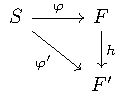
\includegraphics[scale=1.5]{images/fig_6.pdf}\\
                Figura \thefigcount. Isomorfismo entre $F$ y $F'$.
                \stepcounter{figcount}
            \end{center}
        \end{minipage}

        es conmutativo
    \end{propo}

    \begin{proof}
        El procedimiento es análogo al de la proposición \ref{caractSumDir_2}.
    \end{proof}

    De momento, no hemos dicho que dado un conjunto $S$, existe un grupo abeliano libre $F$ en $S$. Nuestra tarea será de probar la existencia de este grupo abeliano libre en $S$.

    \begin{propo}
        \label{caracProdFreeAbelian}
        Suponga que $\left\{S_i \right\}_{i\in I}$ es una familia de subconjuntos de $S$ no vacíos, que son disjuntos a pares para los que se cumple que:
        \begin{equation*}
            S=\bigcup_{ i\in I}S_i
        \end{equation*}
        para cada $i\in I$, sea $F_i$ un grupo abeliano libre en $S_i$ con respecto a la función $\cf{\varphi_i}{S_i}{F_i}$. Sea
        \begin{equation*}
            F=\bigoplus_{ i\in I}F_i
        \end{equation*}
        (esto es, $F$ es el producto débil de los $F_i$, o la suma directa de los mismos). Entonces, si $\cf{\eta_i}{F_i}{F}$ es el monomorfismo natural, se define $\cf{\varphi}{S}{F}$ dada por:
        \begin{equation*}
            \varphi(x)=\eta_i\circ\varphi_i(x),\quad\textup{ si }x\in S_i\textup{ para algún }i\in I
        \end{equation*}
        Entonces, $F$ es un grupo abeliano libre en $S$ con respecto a la función $\varphi$.
    \end{propo}

    \begin{proof}
        Sea $A$ un grupo abeliano y sea $\cf{\psi}{S}{A}$ una función. Para cada $i\in I$, sea
        \begin{equation*}
            \psi_i=\psi\big|_{S_i}
        \end{equation*}
        Como $F_i$ es grupo abeliano libre en $S_i$ con respecto a $\varphi_i$, entonces existe un único homomorfismo $\cf{f_i}{F_i}{A}$ tal que el diagrama
        
        \begin{minipage}{\textwidth}
            \begin{center}
                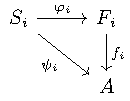
\includegraphics[scale=1.5]{images/fig_7.pdf}\\
                Figura \thefigcount. Propiedad Universal $F_i$ y $A$ .
                \stepcounter{figcount}
            \end{center}
        \end{minipage}

        es conmutativo, para todo $i\in I$. Considere la familia de funciones $\left\{f_i \right\}_{i\in I}$. Por el Teorema \ref{caractSumDir_1}, existe un único homomorfismo tal que el diagrama

        \begin{minipage}{\textwidth}
            \begin{center}
                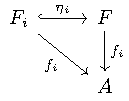
\includegraphics[scale=1.5]{images/fig_8.pdf}\\
                Figura \thefigcount. Conmutatividad de $F_i$, $F$ y $A$ .
                \stepcounter{figcount}
            \end{center}
        \end{minipage}

        es conmitativo para todo $i\in I$. Se sigue que al tenerse
        \begin{equation*}
            \varphi\big|_{S_i}=\eta_i\circ\varphi_i,\quad\forall i\in I
        \end{equation*}
        se tiene que el diagrama

        \begin{minipage}{\textwidth}
            \begin{center}
                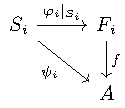
\includegraphics[scale=1.5]{images/fig_9.pdf}\\
                Figura \thefigcount. Conmutatividad de $S_i$, $F$ y $A$ .
                \stepcounter{figcount}
            \end{center}
        \end{minipage}

        es conmutativo, para todo $i\in I$. Como $\psi_i=\psi$ y $S=\bigcup_{i\in I}S_i$, se sigue que:
        \begin{equation*}
            \psi=f\circ\varphi
        \end{equation*}
        (es decir, que el diagrama anterior sin las $i$'s es conmutativo).

        Ahora, probaremos que la $f$ es única. Sea $\cf{f}{F}{A}$ un homomorfismo tal que
        \begin{equation*}
            \psi=f\circ\varphi
        \end{equation*}
        defina $\cf{f_i}{F_i}{A}$ como $f_i=\eta_i\circ f$. Se sigue:
        \begin{equation*}
            \begin{split}
                f_i\circ\varphi_i&=(f\circ\eta_i)\circ\varphi_i\\
                &=f\circ(\eta_i\circ\varphi_i)\\
                &=f\circ\varphi\big|_{S_i}\\
                &=(f\circ \varphi)\big|_{S_i}\\
                &=\psi\big|_{S_i}\\
                &=\psi_i\\
            \end{split}
        \end{equation*}
        como $F_i$ es grupo libre en $S_i$ respecto a $\varphi_i$, se sigue que cada $f_i$ es única, luego $f$ es única (pues queda caracterizada por sus reestricciones a cada $S_i$, es decir, por cada $f_i$).

        Por tanto, $F$ es grupo abeliano libre en $S$ con respecto a $\varphi$.
    \end{proof}

    En términos generales, lo que esta proposición nos dice es que el producto débil de cualquier colección de grupos abelianos libres sigue siendo un grupo abeliano libre.

    \begin{mydef}
        Sea $a$ una letra. Se definen las \textbf{potencias de $a$} como:
        \begin{equation*}
            a^n=\underset{n-\textup{veces}}{\underbrace{a\cdots a}}
        \end{equation*}
        si $n=1$, simplemente se escribirá $a$ en vez de $a^1$. Lo que estamos haciendo es concatenar la letra $a$ $n-$veces consigo misma. Además, se define la letra $a^{0}$ como aquella tal que
        \begin{equation*}
            a^0b=ba^0=b
        \end{equation*}
        para toda letra $b$. Finalmente, se define el \textbf{inverso de $a$} denotado por $a^{-1}$ como la letra tal que
        \begin{equation*}
            a^{-1}a=aa^{-1}=b^{0}
        \end{equation*}
        para toda letra $b$.
    \end{mydef}

    \begin{obs}
        Piense en una letra como literlmente una forma de ver letras en el contexto matemático, haciendo las operaciones de concatenación de letras. Concatenar dos letras significa formar una palabra. Esta terminología es usual en la parte de grupos libres.

        Con estas letras, se generearán grupos abelianos y no abelianos, cosa que se verá más adelante.
    \end{obs}

    \begin{mydef}
        Sea $a$ una letra. Entonces, el conjunto
        \begin{equation*}
            A=\left\{a^m\Big|m\in\mathbb{Z} \right\}
        \end{equation*}
        es un grupo con respecto a la operación concatenación de las potencias de $a$ consigo misma, el cual es un grupo cíclico libre con generador $a$.
    \end{mydef}

    \begin{proof}
        Observemos primero que, si $a^i,a^j\in A$, entonces:
        \begin{equation*}
            \begin{split}
                a^i\cdot a^j&=(\underset{i-\textup{veces}}{\underbrace{a\cdots a}})(\underset{j-\textup{veces}}{\underbrace{a\cdots a}})\\
                &=\underset{(i+j)-\textup{veces}}{\underbrace{a\cdots a}}\\
                &=a^{ i+j}\\
            \end{split}
        \end{equation*}
        en caso de que algún $i$ o $j$ sea negativo, se tiene que:
        \begin{equation*}
            \underset{i-\textup{veces}}{\underbrace{a\cdots a}}=\underset{\abs{i}-\textup{veces}}{\underbrace{a^{-1}\cdots a^{-1}}}
            =\underset{(-i)-\textup{veces}}{\underbrace{a^{-1}\cdots a^{-1}}}
        \end{equation*}
        así que, la operación concatenación de $A\times A$ en $A$ está bien definida. Se verifica rápidamente que $A$ es grupo con esta operación, con elemento identidad $a^0$ y para cada $a^i\in A$, su inverso está dado por:
        \begin{equation*}
            (a^i)^{-1}=a^{-i}
        \end{equation*}

        Es inmediato que $A$ es abeliano y que es cíclico generado por $a$.
    \end{proof}

    \begin{propo}
        \label{freeAbelianOneGroup}
        Sea $x$ una letra y defina $S=\left\{x \right\}$. Entonces, el grupo
        \begin{equation*}
            F=\left\{x^m\Big|m\in\mathbb{Z} \right\}
        \end{equation*}
        es un grupo abeliano libre en $S$ con respecto a la función $\cf{\varphi}{S}{F}$ dada por:
        \begin{equation*}
            \varphi(x)=x^1=x
        \end{equation*}
    \end{propo}

    \begin{proof}
        Sea $A$ un grupo abeliano y $\cf{\psi}{S}{A}$ una función. Sea $\cf{f}{F}{A}$ la función dada por:
        \begin{equation*}
            f(x^m)=\psi(x)^m,\quad\forall x\in\mathbb{Z}
        \end{equation*}
        Es claro que $f$ es homomorfismo entre $F$ y $A$. Se cumple además que:
        \begin{equation*}
            \begin{split}
                f\circ\varphi(x)&=f(x)\\
                &=\psi(x)\\
                \Rightarrow f\circ\varphi&=\psi\\
            \end{split}
        \end{equation*}
        Veamos que es único. Si $\cf{g}{F}{A}$ es otro homomorfismo entre $F$ y $A$ tal que
        \begin{equation*}
            g\circ\varphi=\psi
        \end{equation*}
        se tiene que
        \begin{equation*}
            g\circ\varphi(x)=\psi(x)\Rightarrow g(x)=\psi(x)
        \end{equation*}
        por lo que:
        \begin{equation*}
            \begin{split}
                f(x^m)&=\psi(x)^m\\
                &=g(x)^m\\
                &=g(x^m),\quad\forall m\in\mathbb{Z} \\
            \end{split}
        \end{equation*}
        por ser $g$ homomorfismo. Por tanto, $f=g$.

        Así, $F$ es un grupo abeliano libre en $S$ con respecto a $\varphi$.
    \end{proof}

    \begin{exa}
        $\mathbb{Z}$ es un grupo abeliano libre en $\left\{1 \right\}$.
    \end{exa}

    \begin{propo}
        Sea $S$ un conjunto. Entonces, existe un grupo abeliano libre $F$ en $S$ con respecto a alguna función $\cf{\varphi}{S}{F}$.
    \end{propo}

    \begin{proof}
        Podemos considerar que los elementos de $S$ son letras (a cada elemento de $S$ le podemos asociar una letra, digamos $x_i$). Por lo que, podemos escribir $S$ como:
        \begin{equation*}
            S=\left\{x_i\Big|i\in I \right\}
        \end{equation*}
        (donde $x_i\neq x_j$ para todo $i,j\in I$, $i\neq j$). Sea $S_i=\left\{x_i \right\}$ para todo $i\in I$. Entonces, el grupo abeliano
        \begin{equation*}
            F_i=\left\{x_i^m\Big|m\in\mathbb{Z} \right\}
        \end{equation*}
        es un grupo abeliano libre en $S_i$ con respecto a $\cf{\varphi_i}{S_i}{F_i}$ dada por:
        \begin{equation*}
            \varphi_i(x_i)=x_i
        \end{equation*}
        esto por la Proposición anterior. Ahora, por la Proposición \ref{caracProdFreeAbelian}, se tiene que $S$ es un grupo abeliano libre en $F$ con respecto a $\varphi$, siendo
        \begin{equation*}
            F=\bigoplus_{ i\in I}F_i
        \end{equation*}
        la suma directa (o el producto débil) de los $F_i$, y $\cf{\varphi}{S}{F}$ la función dada por:
        \begin{equation*}
            (\varphi(x_i))(j)=\left\{
                \begin{array}{lcr}
                    x_i^1 & \textup{ si } & i=j\\
                    x_j^0 & \textup{ si } & i\neq j\\
                \end{array}
            \right.
        \end{equation*}
        (recuerde que $\varphi(x_i)$ es una función de $I$ en la unión de los $F_i$).
    \end{proof}

    \begin{obs}
        De la proposición anterior, se sigue que $\varphi$ es inyectiva. Por lo que, podemos identificar cada elemento $x_i\in S$ con su imagen $\varphi(x_i)\in F$. Así que hacemos el abuso de notación:
        \begin{equation*}
            \varphi(x_i)=x_i
        \end{equation*}
        Por lo que, $S$ podemos verlo como subconjunto de $F$ y, de forma inmediata se ve que podemos expresar cada elemento $g\in F$ diferente de la identidad de $F$ como:
        \begin{equation*}
            g=x_{ i_1}^{ n_1}x_{ i_2}^{ n_2}\cdots x_{ i_k}^{ n_k}
        \end{equation*}
        donde $i_1,i_2,...,i_k\in I$ y $n_1,n_2,...,n_k$ son enteros no cero. Esta expresión de $g$ es única, salvo el orden de los factores. Más aún, cada producto de este tipo representa de forma única a un elemento de $F$. Por lo tanto, se puede demostrar rápidamente (vea el primer ejercicio), que $F$ es generado por $S=\varphi(S)$.
    \end{obs}

    Identificar a $S$ con $\varphi(S)$ es muy común en la literatura. Cuando se haga esto, el mapeo $\cf{\varphi}{S}{F}$ se convierte en una inyección, por lo que usualmente no se menciona.

    \begin{propo}
        Cualquier grupo abeliano libre es la imagen homeomorfa de un grupo abeliano libre. Esto es, dado un grupo abeliano $A$ existe un grupo abeliano libre $F$ y un epimorfismo $\cf{f}{F}{A}$.
        
        Más aún, todo grupo abeliano es isomorfo al cociente de un grupo abeliano libre con un subgrupo normal del mismo.
    \end{propo}

    \begin{proof}
        Sea $A$ un grupo abeliano. Sea $S\subseteq A$ un conjunto no vacío que genera a $A$, esto es: $A=\langle S\rangle$.

        Sea ahora $F$ un grupo abeliano libre en $S$ con respecto a $\cf{\varphi}{S}{F}$ función inyectiva. Considere $\cf{\psi}{S}{A}$ dada por:
        \begin{equation*}
            \psi(s)=s,\quad\forall s\in S
        \end{equation*}
        Entonces, como $F$ es grupo abeliano libre en $S$, existe un único homomorfismo $\cf{f}{F}{A}$ tal que
        \begin{equation*}
            f\circ\varphi=\psi
        \end{equation*}
        Afirmamos que $f$ es epimorfismo. Sea $a\in A$, entonces existen $s_1,...,s_k\in S$ diferentes entre sí y $n_1,...,n_k\in\mathbb{Z}$ no cero tales que:
        \begin{equation*}
            a=s_1^{n_1}\cdots s_k^{n_k}
        \end{equation*}
        Por tanto, como podemos ver a $S$ como subconjunto de $F$, podemos tomar el elemento $s_1^{n_1}\cdots s_k^{n_k}\in F$, el cual es tal que:
        \begin{equation*}
            \begin{split}
                f\left(s_1^{n_1}\cdots s_k^{n_k}\right)&=f(s_1)^{ n_1}\cdots f(s_k)^{ n_k}\\
                &=f\circ\varphi(s_1)^{ n_1}\cdots f\circ\varphi(s_k)^{ n_k}\\
                &=\psi(s_1)^{ n_1}\cdots\psi(s_k)^{ n_k}\\
                &=s_1^{n_1}\cdots s_k^{n_k}\\
                &=a\\
            \end{split}
        \end{equation*}
        por tanto, $f$ es epimorfismo.
        
        Para la segunda parte, se tiene por el Primer Teorema de Isomorfismos, se tiene que
        \begin{equation*}
            F/\ker f\cong A
        \end{equation*}
        donde $\ker f$ es un subgrupo normal de $F$.
    \end{proof}

    \begin{obs}
        $F$ y $A$ no son el mismo conjunto. Recuerde que $F$ se construye por concatenación de letras, por lo que el orden de todo elemento de $F$ es infinito, mientras que puede que no todo elemento de $A$ sea de orden infinito.
    \end{obs}

    Con esta proposición, se hace más sencillo dar una definición precisa de una relación no trivial entre los elementos de $A$.

    \begin{mydef}
        Sean $A$, $S$, $F$ y $\cf{f}{F}{A}$ como en la definición anterior. Un elemento $r\in F$ diferente de la identidad es una \textbf{relación no trivial} entre el conjunto de generadores de $S$, si $r\in\ker f$.

        Si $\left\{r_i \right\}_{ i\in I}$ es una colección cualquiera de relaciones no triviales, y $r$ es un elemento de
        \begin{equation*}
            \langle r_i\Big|i\in I \rangle
        \end{equation*}
        entonces se dice que $r$ es una \textbf{consecuencia de $\left\{r_i \right\}_i\in I$}.
    \end{mydef}

    Si la colección $\left\{r_i \right\}_{ i\in I}$ genera el kernel de $f$, entonces el grupo $A$ está totalmente determinado (hasta isomorfismos) por $S$ y las relaciones $\left\{ r_i \right\}_{ i\in I}$. En este caso, se tiene que:
    
    \begin{equation*}
        A\cong F/\langle r_i\Big|i\in I \rangle
    \end{equation*}

    \begin{obs}
        Si $r$ es consecuencia de $\left\{r_i \right\}_{ i\in I}$, entonces $r$ puede ser expresado como el producto de algunos $r_i$ junto con sus inversos.
    \end{obs}

    \begin{propo}
        Sean $S$ y $S'$ conjuntos con la misma cardinalidad y, $F$ y $F'$ grupos abelianos libres en $S$ y $S'$, respectivamente. Entonces, $F\cong F'$.
    \end{propo}

    \begin{proof}
        Como $F$ y $F'$ son grupos abelianos libres en sus respectivos conjuntos, existen funciones $\cf{\varphi}{S}{F}$ y $\cf{\varphi'}{S'}{F'}$ inyectivas.

        Como $\abs{S}=\abs{S'}$, entonces existe una biyección $\cf{h}{S}{S'}$. Así, $\cf{\psi'=\varphi\circ h^{-1}}{S'}{F}$ y $\cf{\psi=\varphi'\circ h}{S}{F'}$ son funciones de $S$ en $F'$ y $S'$ en $F$, respectivamente. Por tanto, existen únicos homomorfismos $\cf{f}{F}{F'}$ y $\cf{g}{F'}{F}$ tales que:
        \begin{equation*}
            f\circ \varphi=\psi\quad\textup{y}\quad g\circ\varphi'=\psi'
        \end{equation*}
        luego,
        \begin{equation*}
            f\circ\varphi\circ h^{-1}=\varphi'\quad\textup{y}\quad g\circ\varphi'\circ h=\varphi
        \end{equation*}
        por lo cual, sustituyendo $\varphi$ en la primer ecuación y a $\varphi'$ en la segunda, se sigue que:
        \begin{equation*}
            f\circ g\circ\varphi'=\varphi'=\bbm{1}_{F'}\circ\varphi' \quad\textup{y}\quad g\circ f\circ\varphi=\varphi=\bbm{1}_{F}\circ\varphi
        \end{equation*}
        Siendo las funciones $f$ y $g$ únicas, debe suceder que:
        \begin{equation*}
            f\circ g=\bbm{1}_{ F'}\quad\textup{y}\quad g\circ f=\bbm{1}_{ F}
        \end{equation*}
        así, $f$ es isomorfismo con inversa $g$. Luego $F\cong F'$
    \end{proof}

    Resulta que en la proposición anterior, el converso es verdadero (al menos en el caso finito).

    \begin{mydef}
        Sea $G$ un grupo y $n\in\mathbb{Z}$. Entonces, el conjunto $G^n$ denota al subgrupo generado por $\left\{g^n\Big|g\in G \right\}$. En el caso en que $G$ sea abeliano, se tiene que:
        \begin{equation*}
            G^n=\langle g^n\Big|g\in G\rangle=\left\{g^n\Big|g\in G \right\}
        \end{equation*}
    \end{mydef}

    \begin{lema}
        Sea $F$ un grupo abeliano libre en un conjunto de $k\in\mathbb{N}$ elementos. Entonces, dado $n\in\mathbb{N}$, el grupo cociente $F/F^n$ es un grupo finito de orden $n^k$.
    \end{lema}

    \begin{proof}        
        Sea $n\in\mathbb{N}$. Es claro que $F/F^n$ es grupo (por ser $F$ abeliano y $F^n$ subgrupo del mismo). Podemos suponer que $F$ es libre en $S$, dado por:
        \begin{equation*}
            S=\left\{x_0,...,x_{ k-1} \right\}
        \end{equation*}
        y, hacemos $x_k=x_0$. Considere a $S$ como subconjunto de $F$. 
        
        %TODO Hay que hacer algo con productos finitos de $S$
        
        Sea ahora $\cf{f}{\natint{1,2,...,n^k}}{F/F^n}$ dada por:
        \begin{equation*}
            f(m)=F^nx_{\lfloor\log_n m \rfloor}^{r}
        \end{equation*}
        donde $0\leq r<n$ es tal que $r\equiv m\bmod n$. Claramente $f$ está bien definida (se verifica rápidamente, pues $0\leq\lfloor\log_nm\rfloor\leq k$ para todo $m\in\natint{1,...,n^k}$). Es inmediato que esta función es inyectiva, veamos que es suprayectiva.

        Sea $a\in F$, entonces existen $n_1,...,n^k\in\mathbb{Z}$ tales que:
        \begin{equation*}
            a=x_1^{ n_1}\cdots x_k^{ n_k}
        \end{equation*}
        sean $r_1,...,r_n$
    \end{proof}

    \begin{cor}
        Sean $S$ y $S'$ conjuntos finitos con cardinales distintos, y sean $F$ y $F'$ grupos abelianos libres en $S$ y $S'$, respectivamnete. Entonces, $F$ y $F'$ no son isomorfos.
    \end{cor}

    \begin{proof}
        Como $S$ y $S'$ tienen cardinales distintos, entonces $F/F^2$ y $F'/F'^{ 2}$ tienen cardinalidad distinta, en particular, no puede suceder que $F$ y $F'$ sean isomorfos.
    \end{proof}

    \begin{cor}
        Sean $F$ y $F'$ grupos libres isomorfos en $S$ y $S'$, respectivamente. Entonces, $\abs{S}=\abs{S'}$.
    \end{cor}

    \begin{proof}
        Inmediata del corolario anterior.
    \end{proof}

    Básicamente hemos caracterizado una propiedad fundamental de los grupos libres en un conjunto dado $S$, la cual se enuncia en la siguiente definición.

    \begin{mydef}
        Sea $F$ un grupo abeliano libre en un conjunto $S$ finito. El cardinal de $S$ es llamado el \textbf{rango de $F$}.
    \end{mydef}

    \section{Productos Libres de Grupos}

    El producto libre de una colección arbitraria de grupos $G_i$ (no necesariamente todos abelianos) es el análogo al producto débil para grupos abelianos.

    El objetivo de esto es definir de forma análoga a como se hizo anteriormente, un grupo libre, esto se hace prescindiendo del grupo de palabras, sin embargo, como notará su construcción es exactamente la misma.

    \begin{mydef}
        Sea $\left\{G_i \right\}_{ i\in I}$ una colección no vacía de grupos. Suponga que existe un grupo $G$ tal que para todo $i\in I$, está dado un homomorfismo
        \begin{equation*}
            \cf{\varphi_i}{G_i}{G}
        \end{equation*}
        Decimos que $G$ es el \textbf{producto libre} o \textbf{coproducto de los grupos $G_i$ con respecto a los homomorfismos $\varphi_i$}, si se cumple lo siguiente:
        
        \begin{itemize}
            \item Para todo grupo $H$ y cualquier familia de homomorfismos $\left\{\psi_i \right\}_{ i\in I}$ tales que
            \begin{equation*}
                \cf{\psi_i}{G_i}{H},\quad\forall i\in I
            \end{equation*}
            existe un único homomorfismo $\cf{f}{G}{H}$ tal que el diagrama
    
            \begin{minipage}{\textwidth}
                \begin{center}
                    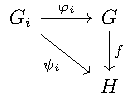
\includegraphics[scale=1.5]{images/fig_10.pdf}\\
                    Figura \thefigcount. Conmutatividad en el producto libre de grupos.
                    \stepcounter{figcount}
                \end{center}
            \end{minipage}
    
            es conmutativo para todo $i\in I$.
        \end{itemize}
    \end{mydef}

    Esta caracterización es tan específica para probar la unicidad y existencia de este producto libre de grupos.

    \begin{propo}
        Suponga que $G$ y $G'$ son productos libres de la familia no vacía de grupos $\left\{G_i \right\}_{ i\in I}$ (con respecto a los homomorfismos $\cf{\varphi_i}{G_i}{G}$ y $\cf{\varphi_i'}{G_i}{G'}$, respectivamente). Entonces, existe un único isomorfismo $\cf{h}{G}{G'}$ tal que el siguiente diagrama

        \begin{minipage}{\textwidth}
            \begin{center}
                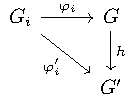
\includegraphics[scale=1.5]{images/fig_11.pdf}\\
                Figura \thefigcount. Conmutatividad entre $G_i$, $G$ y $G'$.
                \stepcounter{figcount}
            \end{center}
        \end{minipage}

        es conmutativo para todo $i\in I$.
    \end{propo}

    \begin{proof}
        Es una copia de la prueba de la Proposición \ref{caractSumDir_2}. 
    \end{proof}

    A pesar de que hemos definido el producto libre de grupos, no hemos asegurado su existencia. De paso, también deberíamos de mostrar que cada homomorfismo $\varphi_i$ es monomorfismo y más aún, que $G$ es el grupo libre generado por la unión de las imágenes $\varphi(G_i)$ y dar más estructura algebraica del mismo.

    Este será nuestro objetivo de ahora en adelante.

    \begin{mydef}
        Sea $\left\{ G_i \right\}_{ i\in I}$ un conjunto no vacío de grupos. Una \textbf{palabra en la familia $\left\{ G_i \right\}_{ i\in I}$ de longitud $n\in\mathbb{N}$} es una sucesión finita $(x_1,x_2,...,x_n)$ de elementos en $\bigcup_{ i\in I}G_i$ tal que:
        \begin{itemize}
            \item Para todo $j\in\natint{1,n}$ existe $i_j\in I$ tal que $x_j\in G_{ i_j}$.
            \item $x_j\neq e_{ G_i}$ para todo $j\in\natint{1,n}$ y para todo $i\in I$.
            \item Si $n>1$, entonces para todo $j\in\natint{1,n-1}$ se tiene que $x_j$ y $x_{ j+1}$ no están en el mismo grupo.
        \end{itemize}
        $n$ es llamado la \textbf{longitud de la palabra}. Se define además al \textbf{palabra vacía}, como el conjunto vacío $\emptyset$, que se identificará con $(\cdot)$ la cual tiene longitud 0.

        Se denotará por $\mathscr{W}$ al conjunto de todas las palabras de longitud no negativa en $\left\{G_i \right\}_{ i\in I}$.
    \end{mydef}

    \begin{theor}
        Dada una colección no vacía $\left\{ G_i \right\}_{ i\in I}$ de grupos, su producto libre existe.
    \end{theor}
    
    \begin{proof}
        Veamos que $\mathscr{W}$ es el producto libre de la familia $\left\{G_i \right\}_{ i\in I}$. Veamos que $\mathscr{W}$ es grupo con la operación $\cdot$ definida como sigue:
        \begin{equation*}
            (x_1,...,x_n)\cdot(y_1,...,y_m)=\left\{
                \begin{array}{lcr}
                    (x_1,...,x_n,y_1,...,y_m) & \textup{ si } & x_n\textup{ y }y_1\textup{ no están en el mismo }G_i\\
                    (x_1,...,x_ny_1,...,y_m) & \textup{ si } & x_n\textup{ y }y_1\textup{ en el mismo }G_i\textup{ y }x_ny_1\neq e_i\\
                    (x_1,...,x_{ n-1},y_2,...,y_m) & \textup{ si } & x_n\textup{ y }y_1\textup{ en el mismo }G_i\textup{ y }x_ny_1= e_i\\
                \end{array}
            \right.
        \end{equation*}
        hace de $\mathscr{W}$ un grupo. En efecto, claramente esta operación es asociativa, el elemento identidad es $(\cdot)$ y el inverso de una palabra $(x_1,...,x_n)$ es $(x_n^{-1},...,x_1^{-1})$.

        Sea $i\in I$, se define el homomorfismo $\cf{\varphi_i}{G_i}{\mathscr{W}}$ dado por:
        \begin{equation*}
            \varphi_i(g)=\left\{
                \begin{array}{lcr}
                    (g) & \textup{ si } & g\neq e_i\\
                    (\cdot) & \textup{ si } & g= e_i\\
                \end{array}
            \right.,\quad\forall g\in G_i
        \end{equation*}
        (claramente éste es homomorfismo, más aún es monomirfismo. Veamos ahora que $\mathscr{W}$ es el producto libre de los grupos $G_i$.

        Sea $H$ un grupo y $\left\{\cf{\psi_i}{G_i}{H} \right\}_{ i\in I}$ una familia de homomorfismos. Defina el homomorfismo $\cf{f}{\mathscr{W}}{H}$ dado por:
        \begin{equation*}
            f(x_1,....,x_n)=\psi_{i_1}(x_1)\cdots\psi_{i_n}(x_n)
        \end{equation*}
        para toda palabra no vacía, y $f(\cdot)=e_H$ (donde $e_H\in H$ es la identidad del grupo), donde $x_j\in G_{i_j}$ para todo $j=1,...,n$.
        
        Claramente este es homomorfismo y está bien definido, veamos que para $i\in I$:
        \begin{equation*}
            \begin{split}
                f\circ\varphi_i(g)&=f(g)\\
                &=\psi_i(g)\\
            \end{split}
        \end{equation*}
        (recuerde que en el segundo lado de la primera igualdad estamos evaluando a $f$ en la palabra $(g)$), para todo $g\in G_i$ diferente de la identidad, y:
        \begin{equation*}
            \begin{split}
                f\circ\varphi_i(e_i)&=f(\cdot)\\
                &=e_H\\
                &=\psi_i(e_i)\\
            \end{split}
        \end{equation*}
        por lo que:
        \begin{equation*}
            f\circ\varphi_i=\psi_i
        \end{equation*}
        Veamos que es único. Sea $\cf{g}{\mathscr{W}}{H}$ otro homomorfismo tal que:
        \begin{equation*}
            g\circ\varphi_i=\psi_i,\quad\forall i\in I
        \end{equation*}
        Si $(x_1,...,x_n)\in\mathscr{W}$ es una palabra, se tiene que:
        \begin{equation*}
            \begin{split}
                g(x_1,...,x_n)&=g((x_1)\cdot(x_2)\cdots(x_n))\\
                &=g((x_1))\cdots g((x_n))\\
                &=g\circ\varphi_{i_1}(x_1)\cdots g\circ\varphi_{i_n}(x_n)\\
                &=\psi_{ i_1}(x_1)\cdots\psi_{ i_n}(x_n)\\
                &=f(x_1,...,x_n)
            \end{split}
        \end{equation*}
        donde $x_j\in G_{ i_j}$ para todo $j=1,...,n$. Así que $g=f$.

        Por ende, se sigue que $\mathscr{W}$ es el producto libre de la familia $G_i$.
    \end{proof}

    \begin{obs}
        Dos hechos importantes del teorema anterior son los siguientes:
        \begin{enumerate}[label = \textit{(\alph*)}]
            \item Cuando $G_i\neq G_j$ para todo $i\neq j$, se tiene que cualquier elemento $g$ del producto libre de los $G_i$ se expresa de forma única como producto de elementos de los $G_i$.
            \item Es natural la forma en la que se definió el producto de las palabras en $\mathscr{W}$.
        \end{enumerate}
    \end{obs}

    \begin{exa}
        Sean $G_1$ y $G_2$ grupos cíclicos de orden 2, digamos $G_1=\left\{1,x_1 \right\}$ y $G_2=\left\{1,x_2 \right\}$ con $x_1\neq x_2$. Entonces, todo elemento distinto de la identidad en el producto libre de $G_1$ por $G_2$ se expresa de forma única como producto de $x_1$ por $x_2$, alternando cada uno de éstos. Por ejemplo, los siguientes elementos:
        \begin{equation*}
            x_1,x_1x_2,x_1x_2x_1,x_1x_2x_1x_2,...
        \end{equation*}
        o,
        \begin{equation*}
            x_2,x_2 x_1,x_2x_1x_2,x_2x_1x_2x_1,...
        \end{equation*}

        Note que los elementos $x_1x_2$ y $x_2x_1$ tienen orden infinito y son diferentes. Esta es una diferencia muy grande con respecto al producto débil de $G_1$ con $G_2$, ya que el producto directo de estos dos grupos es un grupo de orden 4, mientras que el producto libre es de orden infinito.
    \end{exa}

    \begin{mydef}
        Sea $\left\{G_i \right\}_{ i\in I}$ una familia de grupos.
        \begin{itemize}
            \item Si la familia es finita, digamos $G_1,...,G_n$, denotamos el producto libre de la familia por $G_1*G_2*\cdots*G_n$, o también como:
            \begin{equation*}
                {\prod_{ 1\leq i\leq n}}^*G_i
            \end{equation*}
            \item En general, el producto libre de la familia $\left\{G_i \right\}_{ i\in I}$ se denota por:
            \begin{equation*}
                {\prod_{ i\in I}}^*G_i
            \end{equation*}
        \end{itemize}
    \end{mydef}
    
    \section{Grupos Libres}

    \begin{exa}
        El grupo diédrico $D_n$, se define como
        \begin{equation*}
            D_n=\langle a,b\Big|a^n=1,b^2=1,ba=a^{n-1}b \rangle
        \end{equation*}
        (en este caso, no conmutan los elementos).
    \end{exa}

    \newpage

    \section{Ejercicios}

    \begin{excer}
        Pruebe directo de la definición que $\varphi(S)$ genera a $F$.

        \textit{Sugerencia.} Suponga que no, considere el subgrupo $F'$ generado por $\varphi(S)$.
    \end{excer}

    \begin{proof}
        Sea
        \begin{equation*}
            F'=\langle\varphi(S)\rangle
        \end{equation*}
        se tiene que $F'\subseteq F$ y $F'$ es un grupo abeliano. Considere la función
        \begin{equation*}
            \cf{\psi}{S}{F'},\psi(s)=\varphi(s),\quad\forall s\in S
        \end{equation*}
        claramente esta función está bien definida. Por la definición de grupo abeliano libre existe un único homomorfismo $\cf{f}{F}{F'}$ tal que
        \begin{equation*}
            f\circ\varphi=\psi
        \end{equation*}
        esto es que:
        \begin{equation*}
            f\circ\varphi=\bbm{1}_{F'}\circ\varphi
        \end{equation*}
        por tanto, de la unicidad de $f$ se sigue que $f=\bbm{1}_{F'}$, es decir que $F=F'$.

        Por tanto, $\varphi(S)$ genera a $F$.
    \end{proof}

    \begin{excer}
        Pruebe que el Corolario 2.2.1 es cierto si $S$ es finito y $S'$ es infinito.
    \end{excer}
    
    \begin{proof}
        
    \end{proof}

    %TODO: Escribir los ejercicios de la parte de producto libre de grupos.
    
    \begin{excer}[Nombre]
        
    \end{excer}

\end{document}